Using neural networks to learn (potentially high-dimensional) functions constrained by physical laws is a popular trend in scientific machine learning \cite{carleo2017solving, pfau2020ab, hermann2020deep, karniadakis2021physics, raissi2019physics, hu2023hutchinson, sun2020global}.
Typically, the Physics is encoded through partial differential equations (PDEs) the neural net must satisfy.
The associated loss functions require evaluating differential operators \wrt the network's input, rather than weights, which contain higher-order derivatives.
Typically, evaluating the differential operator is a bottleneck.

\paragraph{Differential operators in the wild.} Two important fields of application are variational Monte-Carlo (VMC) and Physics-informed neural networks (PINNs).
VMC employs neural networks as ansatz for the Schr\"odinger equation \cite{carleo2017solving, pfau2020ab, hermann2020deep} and demands computing the net's Laplacian (the Hessian trace) to capture the kinetic energy in the Hamiltonian.
PINNs also use a neural net ansatz to learn a PDE solution and cast the problem as optimization tasks by minimizing the residuals of the governing equations \cite{raissi2019physics, karniadakis2021physics}.
This approach necessitates differentiable application of potentially high-order PDE operators.
For instance, the PINN formulation of Kolmogorov-type equations—including the Fokker-Planck, Black-Scholes, and Hamilton-Jacobi-Bellman equations—requires the evaluation of weighted second-order input derivatives in high-dimensional spatial domains \cite{hu2023hutchinson, sun2024dynamical}.
The Bi-Laplacian is often used for plate equations and contains fourth-order derivatives \todo{Improve sentence, add ref}.

\paragraph{Is backpropagation all we need?}
Although it is known---at least on paper---that nesting first-order automatic differentiation (AD) to compute high-order derivatives scales poorly, this approach is common practise.
The AD community has developed a more favourable alternative to nested backpropagation that promises faster computation of higher-order derivatives: \emph{Taylor-mode AD}~\cite[or simply \emph{Taylor-mode},][\S13]{griewank2008evaluating}.
\citet{bettencourt2019taylor} introduced Taylor-mode to the machine learning community in \citeyear{bettencourt2019taylor} and provided an implementation in JAX \cite{bradbury2018jax}.
However, we observe empirically that vanilla Taylor-mode is often not enough to beat nested backpropagation: We took a 5-layer $\tanh$ activated MLP (such nets are commonly used as PINNs) and evaluated its Laplacian using JAX's Taylor mode and compared its performance to computing, then tracing, the Hessian via Hessian-vector products \cite{pearlmutter1994fast,dagreou2024how}.
On this example, we found that \emph{vanilla Taylor mode is 50\% slower than nested backpropagation}.
This calls into question the relevance of Taylor mode for computing differential operators that ML practitioners are interested in.

\paragraph{No.}
Although it looks like, at first sight, backpropagation is all we need, recent works have successfully demonstrated the potential of Taylor mode and forward propagation schemes.
For the Laplacian, \citet{li2023forward} developed a special forward propagation framework called the \emph{forward Laplacian} (later generalized to weighted Laplacians \cite{li2024dof}).
Coming back to our example from above, we can see that JAX's forward Laplacian \cite{gao2023folx} outperforms nested backpropagation and is roughly twice as fast.
To stochastically approximate differential operators over extremely high-dimensional domains, \citet{shi2024stochastic} proposed using Taylor mode with carefully chosen randomly sampled directions.
While recent work pointed out a connection between Taylor-mode and the forward Laplacian \cite{dangel2024kroneckerfactored}, it remains unclear what disentangles them, and if efficient forward schemes can also be derived for other differential operators.
Our work changes this.
We make the following contributions:

\begin{figure*}[!t]
  \centering
  \begin{minipage}[b]{0.42\linewidth}
    \centering
    \input{figures/vanilla_taylor_not_enough.tex}

    \caption{\textbf{$\blacktriangle$ Vanilla Taylor mode is not enough to beat nested 1\textsuperscript{st}-order AD.}
      Illustrated for computing the Laplacian of a $\mathrm{tanh}$-activated $50 \!\to\! 768 \!\to\! 768 \!\to\! 512 \!\to\! 512 \!\to\! 1$
      MLP with JAX (+ \texttt{jit}) on GPU (details in \Cref{sec:jax-benchmark}).
      We show how to automatically obtain the specialized forward Laplacian through simple graph transformations of vanilla Taylor mode based on linearity, which could be done by the \texttt{jit} compiler.
    }\label{fig:vanilla-taylor-not-enough}

    \vspace{0.25ex}
    \caption{\textbf{$\blacktriangleright$ Our collapsed Taylor mode directly propagates the sum of highest degree coefficients.}
      Visualized for propagating four $K$-jets through a $\sR^5 \!\to\! \sR^3 \!\to\! \sR$ function ($K=2$ yields the forward Laplacian).
      \Cref{sec:introduction} introduces the notation.}
  \end{minipage}
  \hfill
  \begin{minipage}[b]{0.57\linewidth}
    \centering
    \newcommand{\drawgridrectangle}[4]{%
  \begin{tikzpicture}[scale=#4]
    \pgfmathsetmacro{\ymax}{#1}
    \pgfmathsetmacro{\xmax}{#2}

    % Fill the rectangle
    \fill[#3] (0,0) rectangle (\xmax,\ymax);

    % Draw the border
    \draw[white, line width=#4*3pt] (0,0) rectangle (\xmax,\ymax);


    % Draw vertical grid lines
    \pgfmathsetmacro{\xsteps}{#2}
    \foreach \x in {1,...,\xsteps} {
      \draw[white, line width=#4*3pt] (\x,0) -- (\x,\ymax);
    }

    % Draw horizontal grid lines
    \pgfmathsetmacro{\ysteps}{#1}
    \foreach \y in {1,...,\ysteps} {
      \draw[white, line width=#4*3pt] (0,\y) -- (\xmax,\y);
    }
  \end{tikzpicture}%
}

\newsavebox{\taylorStandard}
\savebox{\taylorStandard}{
  \begin{tikzpicture}
    \matrix [%
    matrix of nodes,%
    ampersand replacement=\&,% to use inside a savebox
    nodes={anchor=center, align=center},%
    column sep=4ex,%
    row sep=1ex,%
    ] (taylor)
    {
      \drawgridrectangle{1}{3}{blue!30}{0.33} \& \drawgridrectangle{1}{2}{blue!30}{0.33} \& \drawgridrectangle{1}{1}{blue!30}{0.33}
      \\[-1.5ex]
      $\vx_0$ \& $\vh_0$ \& $\vg_0$
      \\
      \drawgridrectangle{3}{3}{green!30}{0.33} \& \drawgridrectangle{3}{2}{green!30}{0.33} \& \drawgridrectangle{3}{3}{green!30}{0.33}
      \\[-1.5ex]
      $\{\vx_{1,d}\}$ \& $\{\vh_{1,d}\}$ \& $\{\vg_{1,d}\}$
      \\
      \drawgridrectangle{3}{3}{red!30}{0.33} \& \drawgridrectangle{3}{2}{red!30}{0.33} \& \drawgridrectangle{3}{1}{red!30}{0.33} \& \drawgridrectangle{1}{1}{red!60}{0.33}
      \\[-1.5ex]
      $\{\vx_{2,d}\}$ \& $\{\vh_{2,d}\}$ \& $\{\vg_{2,d}\}$ \& $\sum_d \vg_{2,d}$
      \\
    };

    % draw dependencies
    \pgfmathsetmacro{\K}{3}
    \pgfmathsetmacro{\L}{2}

    \foreach \l in {1,...,\L}{
      \pgfmathsetmacro{\lother}{int(\l+1)}
      \foreach \k in {1,...,\K} {
        \pgfmathsetmacro{\row}{int(2*\k-1)}
        \foreach \kother in {\k,...,\K} {
          \pgfmathsetmacro{\rowother}{int(2*\kother-1)}
          \draw[-Stealth, line width=1pt, white!50!black] (taylor-\row-\l.east) -- (taylor-\rowother-\lother.west);
        }
      }
    }
    \pgfmathsetmacro{\Lstart}{int(\L + 1)}
    \pgfmathsetmacro{\Lend}{int(\L + 2)}
    \pgfmathsetmacro{\rowfinal}{int(2*\K - 1)}
    \draw[-Stealth, line width=1pt, white!50!black] (taylor-\rowfinal-\Lstart.east) -- (taylor-\rowfinal-\Lend.west);
  \end{tikzpicture}
}

\newsavebox{\taylorCollapsed}
\savebox{\taylorCollapsed}{
  \begin{tikzpicture}
    \matrix [%
    matrix of nodes,%
    ampersand replacement=\&,% to use inside a savebox
    nodes={anchor=center, align=center},%
    column sep=4ex,%
    row sep=1ex,%
    ] (taylor)
    {
      \drawgridrectangle{1}{3}{blue!30}{0.33} \& \drawgridrectangle{1}{2}{blue!30}{0.33} \& \drawgridrectangle{1}{1}{blue!30}{0.33}
      \\[-1.5ex]
      $\vx_0$ \& $\vh_0$ \& $\vg_0$
      \\
      \drawgridrectangle{3}{3}{green!30}{0.33} \& \drawgridrectangle{3}{2}{green!30}{0.33} \& \drawgridrectangle{3}{3}{green!30}{0.33}
      \\[-1.5ex]
      $\{\vx_{1,d}\}$ \& $\{\vh_{1,d}\}$ \& $\{\vg_{1,d}\}$
      \\[2ex]
      \drawgridrectangle{1}{3}{red!60}{0.33} \& \drawgridrectangle{1}{2}{red!60}{0.33} \& \drawgridrectangle{1}{1}{red!60}{0.33}
      \\[-1.5ex]
      $\sum_d \vx_{2,d}$ \& $\sum_d \vh_{2,d}$ \& $\sum_d \vg_{2,d}$
      \\[1.1ex]
      \& \&
      \\
    };

    % draw dependencies
    \pgfmathsetmacro{\K}{3}
    \pgfmathsetmacro{\L}{2}

    \foreach \l in {1,...,\L}{
      \pgfmathsetmacro{\lother}{int(\l+1)}
      \foreach \k in {1,...,\K} {
        \pgfmathsetmacro{\row}{int(2*\k-1)}
        \foreach \kother in {\k,...,\K} {
          \pgfmathsetmacro{\rowother}{int(2*\kother-1)}
          \draw[-Stealth, line width=1pt, white!50!black] (taylor-\row-\l.east) -- (taylor-\rowother-\lother.west);
        }
      }
    }
  \end{tikzpicture}
}

\begin{figure*}[!t]
  \centering
  \resizebox{\linewidth}{!}{%
    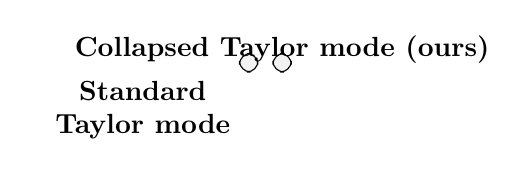
\begin{tikzpicture}
      \node (standard) [fill=black!5!white, draw=black, rounded corners]{\usebox{\taylorStandard}};
      \node [anchor=north east, align=center, inner sep=10pt] at (standard.north east) {\textbf{Standard} \\ \textbf{Taylor mode}};
      \node (collapsed) [fill=black!5!white, draw=black, rounded corners, anchor=north west, xshift=5pt] at (standard.north east) {\usebox{\taylorCollapsed}};
      \node [anchor=south, align=center, inner sep=3pt] at (collapsed.south) {\textbf{Collapsed Taylor mode (ours)}};
    \end{tikzpicture}
  }
  \caption{\textbf{Visual comparison of standard Taylor mode and our proposed collapsed Taylor mode.}}\label{fig:comparison-standard-vs-collapsed}
\end{figure*}

%%% Local Variables:
%%% mode: LaTeX
%%% TeX-master: "../main"
%%% End:

  \end{minipage}
\end{figure*}

\begin{enumerate}[leftmargin=0.5cm]
\item We describe the `collapsed' Taylor mode where the highest Taylor coefficients during the forward propagation are propagated as a weighted sum of said derivatives.
  This approach has first been used in the `forward Laplacian' framework \cite{li2023forward}, which, however, does not rely on Taylor mode.
  Our collapsed Taylor mode improves on it in two ways.
  First, it is based on standard Taylor-mode AD that then allows simple graph rewrites based on linearity.
  Second, it generalizes to other differential operators and can also be applied to recently proposed randomization techniques for Taylor-mode AD.

\item This leads to a conceptually clean separation of concepts, allowing for a simple implementation that can handle all scenarios and does not require manual implementations for each differential operator.
  To demonstrate this, we build a Taylor mode library for PyTorch and equip it with the necessary graph simplifications using the \texttt{torch.fx} library, and show how collapsed Taylor mode accelerates the computation of various differential operators.

\item Ideally, we find specially structured differential operators for which our approach is especially suited and classify them.
  One example is the trace of derivative tensors of arbitrary order, although this seems to be an operator that is not practically relevant.
\end{enumerate}


%%% Local Variables:
%%% mode: LaTeX
%%% TeX-master: "../main"
%%% End:
